\chapter{Rendszerarchitektúra}
\section{Áttekintés}
Ez a fejezet az éles (production) környezet felépítését taglalja.\\
A rendszer 4 szolgáltatásból épül fel:
\begin{description}
    \item[Adatbázis]MySQL 8.0.36 
    \item[PHP-FPM]API (Laravel) kiszolgálása a szerver-kliens kommunikáció megvalósításához
    \item[WebSocket]Node.js és Socket.IO a valós idejű játékmenet megteremtéséhez
    \item[nginx]Frontend kiszolgálása, WebSocket Proxy és FastCGI átjáró biztosítása.
\end{description}
\section{Szolgáltatások és felelősségeik}
\begin{tabular}{l p{14cm}}
    \textbf{Adatbázis} & Biztonságos adattárolás, gyors adatelérés a Laravel EloquentORM használatával. Tranzakciók kezelése, a konzisztencia és adat integritás megőrzése érdekében.\\
    
    \textbf{API} & Biztosítja a szerver és kliens közötti kommunikációt. Lehetővé teszi az üzleti logika tárolását, végrehajtását. Biztonságos autentikáció megvalósítása, HTTP végpontok elérésének biztosítása a kliens számára. Adatbázis-elérés biztosítása az EloquentORM használatával.\\
    
    \textbf{WebSocket} & A valós idejű játékmenet megteremtése. Real time szinkronizáció a Frontend és a Backend között. Megbízható kommunikációs csatorna kiépítése, központosított ideiglenes adattárolás (meccskeresés, aktív játszmák). A WebSocket üzleti logikát nem tartalmaz, és adatbázis-kezelést nem végez.\\
    
    \textbf{nginx} & Frontend kiszolgálása, SSL/TLS kapcsolat kiépítése. WebSocket proxy üzemeltetése valamint FastCGI átjáró a PHP-FPM szolgáltatásnak az api.skillissue.hu virtuális hoszton keresztül.\\
\end{tabular}
\section{Kommunikáció a szolgáltatások között}
A rendszer egy közös Docker hálózatba van bekapcsolva. Ez lehetővé teszi, hogy a szolgáltatások egymást könnyedén elérhessék, a szolgáltatás nevére hivatkozva.
\subsection*{Nginx útvonalválasztás}
Az nginx szerver (1.25) két porton (80, 443) hallgat. Amikor kérés érkezik, megpróbálja kiépíteni a HTTPS (SSL/TLS) kapcsolatot a kliens és a szerver között.\\
Két virtuális hosztot szolgál ki:\\
\textbf{Frontend}: a skillissue.hu frontendet teszi elérhetővé. Emellett be van állítva egy proxy is, a \textit{/socket.io} útvonalra, amely a 3000-res porton hallgató Socket.IO WebSocket szerverre irányít.\\
\textbf{API}: az api.skillissue.hu API-t teszi elérhetővé, amely a FastCGI átjárón keresztül jut el a PHP-FPM szolgáltatáshoz. A PHP-FPM szolgáltatásnak nincsen elérhető portja a külvilág felé, csak a FastCGI vonalon elérhető, csakis az nginx-en keresztül.
\subsection*{Backend és adatbázis}
A Laravel backend PHP-FPM 8.4 alatt fut. Az adatbázis és Laravel közötti kommunikáció az EloquentORM segítségével valósul meg. A MySQL 8.0.36-os verziója a 3306-os porton hallgat, csakis a belső hálózaton, ezáltal kívülről nem elérhető az API megkerülésével. Az adatok tárolására Docker Volume van létrehozva.
\subsection*{API és WebSocket}
A WebSocket és API közötti kommunikációhoz service-to-service token van létrehozva. Ez a kulcs egy közös \texttt{.env} fájlban van tárolva, így mindkét szolgáltatás hozzáfér. Ez a token az \texttt{Authorization} fejlécben kerül elküldésre Bearer tokenként. Ez biztosítja, hogy kizárólag a WebSocket szerver kommunikálhasson közösen az API-val.
\section{Architektúra diagram}
\begin{figure}[h]
    \centering
    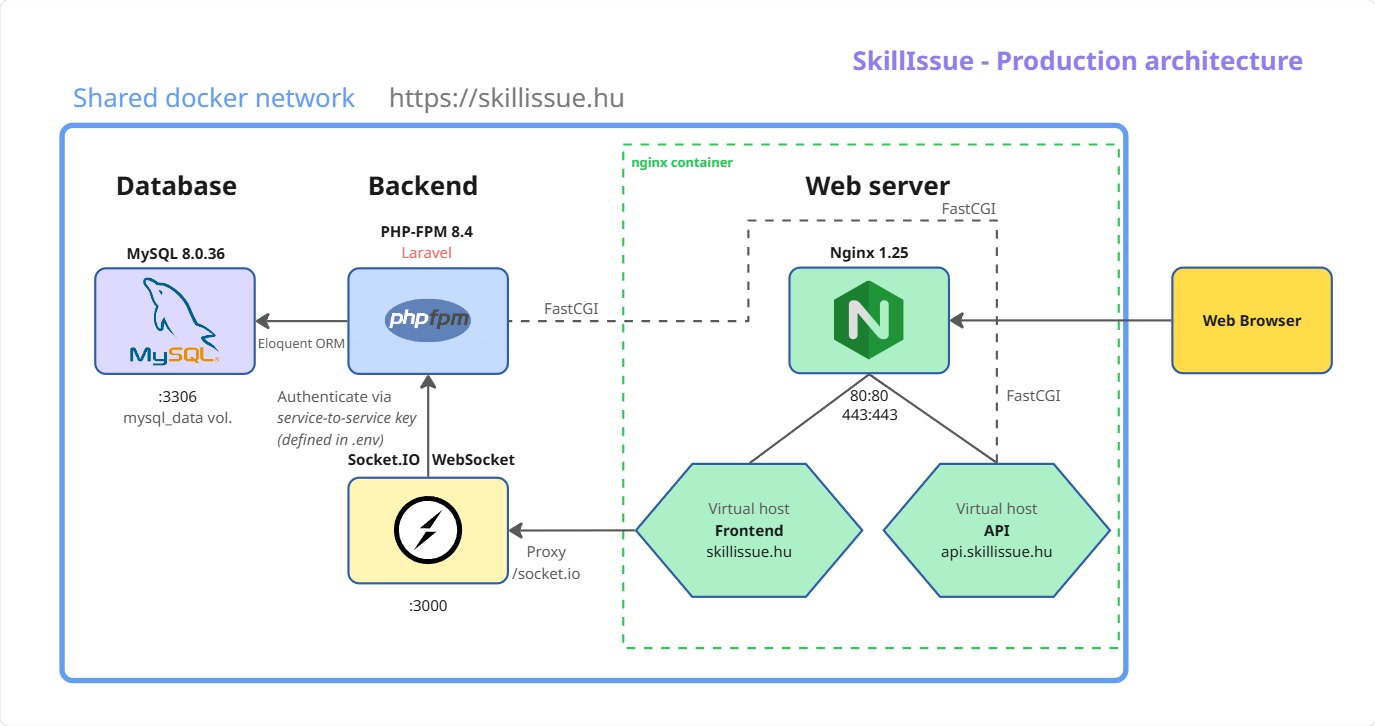
\includegraphics[width=\textwidth]{images/prod_diagram.png}
    \caption{A SkillIssue éles környezetének architektúrája}
    \label{fig:architektura}
\end{figure}